
\section{Background matem\'atico}
\subsection{Combinaci\'ones de distribuci\'ones de probabilidad}
Una operaci'on muy frecuentemente utilizada a lo largo del presente trabajo es la \texttt{combinaci'on convexa} entre distribuciones
de probabilidad.

Dadas $p$ y $q$, dos distribuci'ones de probabilidad sobre el conjunto $S$, y un n'umero $0 \leq \alpha \leq 1$, 
se nota $p +_\alpha q$ a la combinaci'on convexa entre $p$ y $q$, y se define:
$$(p +_\alpha q)(A) = \alpha \times p(A) + (1-\alpha) \times q(A)$$ 

En caso de referirse a $p+q$, se asume que $\alpha = 1/2$. 
\newline \newline
Observaci'ones:
\begin{itemize}
 \item Se puede demostrar que el resultado de combinar dos distribuci'ones de probabilidad de esta forma es tambi'en una distribuci'on 
de probabilidad.

 \item Notar que esta definici'on puede extenderse para $n$ distribuci'ones de probabilidad. En ese caso se necesitar'an valores 
$\alpha_1, \dots, \alpha_n$, tales que $\sum_i \alpha_i = 1$. En general, se utilizara $\alpha_i = 1/n$ salvo que se aclare lo contrario.
\end{itemize}


\subsection{Cadenas de Markov}
Supongamos que se desea modelar la evoluci'on de un sistema con respecto al tiempo. Es de esperarse que 
el estado en el que se encuentra el sistema en cierto momento de alguna forma tenga que ver con la historia por la que este transit'o
previamente. 

Las cadenas de Markov permiten modelar este tipo de dependencias haciendo una asunci'on: el estado en el que se encuentra el sistema
en un momento dado \emph{s'olo} depende del estado anterior en el que este se encontraba. Esta asunci'on es conocida como la propiedad
de falta de memoria.

Formalmente, una cadena de markov es una dupla $<S,P>$, donde $S$ es el conjunto de posibles estados del sistema, y $P$ la 
distribuci'on condicional de ocurrencia, es decir, dados $s_1, s_2 \in S$, el valor de $P(s_2 | s_1)$ indica cual es la probabilidad
de que el sistema pase estado $s_2$ dado que se encuentra actualmente en el estado $s_1$.  Volviendo a la propiedad de falta de memoria, 
ahora es posible expresarla formalmente: $P(s_k | s_1, \cdots s_{k-1}) = P(s_k | s_{k-1})$.

A modo ilustrativo, supongamos que se desea modelar el clima, restringiendo el clima a si llueve o no. De esta forma, el conjunto $S$ de estados
ser'a $\{llueve, no\ llueve\}$. 

Luego de recolectar datos durante un mes, se estiman las siguientes probabilidades:

\begin{center}
\begin{tabular}{l l l l}
$P(lluvia | lluvia) $ & $=0.9$ & $P(lluvia | no\ llueve) $& $=0.1$\\
$P(no\ lluvia | lluvia)  $ & $=0.3$ & $P(no\ lluvia | no\ llueve) $ & $=0.7$\\
\end{tabular}
\end{center}

Gr'aficamente el sistema se ver'ia de la siguiente forma:

\begin{figure}[h]
\begin{center}
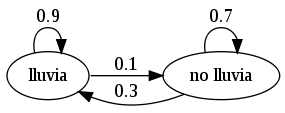
\includegraphics[width=5cm]{images/weather_graph}
\end{center}
\end{figure}


